\chapter{Description logics and biomedical knowledge (Specification)}

\textbf{Key points}
\begin{itemize}
  \item Organisms can be compared to complex black box machines, namely devices with a hidden and unknown internal functioning.
  \item This analogy helps to define the study, needs and representation of biomedical knowledge.
  \item Description logics (DLs), part of a mathematical framework developed to formalise concepts, can be used to study the molecular black box machine and query over recorded biological knowledge. DLs provide the means to represent terms and logically link biological modules.
  \item The framework presented integrates with current life-science information, such as biomedical ontologies (OBO) and databases, and is theoretically highly scalable (\dl{EL\textsuperscript{++}} profile).
  \item The notions introduced and discussed set the groundwork for the representation of the mode of action and the implementation of a new resource built on these principles: The Functional Therapeutic Chemical Classification System (FTC).
\end{itemize}

\textbf{Author’s comment}

This chapter is a summary and record of my experience with the Web Ontology Language (OWL2) and knowledge representation for the biomedical domain. I present a theoretical analysis of the representation of the mode of action and its scalable implementation. A software library to assist the development of programmatic solutions (Brain) is briefly presented in this chapter. I invite the reader to refer to the original publication \citep{croset2013brain} for more detail if wanted.

\hrulefill

\section{Introduction}

Science (from Latin scientia, meaning "knowledge") is a systematic enterprise that builds and organises knowledge in the form of testable explanations and predictions about the universe \citep{sciencewiki}. More specifically, biomedical sciences handle the subset of knowledge related to living organisms. Understanding the biological world is relevant to society as it provides, among other things, some valuable insight to treat and cure diseases. In order for our knowledge to grow, discoveries and evidence have to be recorded, structured and shared with the community and society. Traditionally, biological knowledge is preserved in a narrative fashion, inside textual documents, such as a journal article for example. However, natural language is ambiguous, informal, and impairs an efficient reuse of the information. More recently, with the advent of computer systems, some biological knowledge is stored in a structured way inside databases or ontologies \citep{brooksbank2014european}. Biological entities and concepts have identifiers, enhancing the dissemination and reuse of the information, as well as enabling an efficient integration of multiple datasets. Despite the improvements made towards a more meaningful and consistent representation, I argue that the “logic” in “biologic” is still under-represented. Indeed, it would be valuable to formally derive and prove new facts from existing ones, the same way it is done in algebra for instance. This chapter presents an original approach towards this goal, using description logics (DLs) as a mathematical framework.

In this regard, I first illustrate how the study of organisms is analogous to the theoretical study of a black box machine. From this simple fundamental model and its requirements, I then explain how DLs can, to some extent, capture the internal logic of the cellular machinery. Finally I discuss how this approach can be combined with existing biomedical data, in order to implement automated and scalable solutions. This theoretical work serves as the basis to formally define the concepts of mode and mechanism of action, central points in deriving drug repurposing hypotheses.

\section{Biomedical knowledge}

Life sciences addresses the study of living organisms. Just as in any other scientific discipline, biological researchers first collect data and evidence, which will then be turned into knowledge based on human interpretation \citep{antezana2009biological}. In order to be efficiently reused, understood and shared with the scientific community, some of this knowledge can be represented by a process known as formalisation.

\subsection{Contemporary formalism in biomedical sciences}

Formalism can be described as an abstraction process by the human brain in order to model a system in mathematical terms. Formalising a problem helps to better analyse its complexity. Mathematical models (e.g, equations) are powerful, as they can eventually predict outcomes, once the system is understood well enough. Different scientific disciplines employ different formalisms, depending on the problem studied and research questions being asked.

\subsubsection{Formalism varies among natural sciences}

When I was a college student, I always found biology to differ from other natural sciences such as chemistry or physics for instance. The latter disciplines were built around a particularly strong mathematical scaffold; fundamental phenomena, like the speed of a body, were concisely captured by a function such as $ v=d/t $. Chemical reactions were simplified in the form of an equation such as $ H_{2}O = HO \textsuperscript{-} + H \textsuperscript{+} $ for instance. Despite being approximations of natural processes, these models and equations were useful to learn the discipline. Moreover, once the core concepts were understood, some supplementary layers of complexity were logically added on the top of the known things: Static representations of chemical reactions were transformed into dynamic ones, or it was possible to derive the trajectory of a projectile from its speed and direction, for example.

The formal representation of a system is important, as it clarifies the meaning of the concepts of interest for the community. For instance, speed has a very explicit and clear definition captured by its equation, which can be unambiguously understood and interpreted accordingly. Finally, the most important feature of a formal system is, I believe, that it enables predictions to be made. It becomes possible to infer behaviours and results on the sole basis of the theory. Complex systems can be built and fully understood, relying solely on fundamental principles.

The study of biomedical sciences was not guided by such strong mathematics. Core concepts such as evolution or gene were mostly described in a textual way, a sentence usually defining the meaning; it was impossible to combine concepts in order to create new ones. As biological organisms obey the law of physics and chemistry, one would therefore assume that these frameworks could assist in the study of the living world on their own. They do to some extent; it is for instance possible to represent and model the series of chemical reactions related to a biological pathway using standard chemistry \citep{le2006biomodels}. However, biomedical sciences present particular challenges that cannot adequately be solved by the traditional molecular formalism. First of all, biological bodies are extremely complex from a chemical perspective, either in terms of size or types of compound present (3 x 10\textsuperscript{27} atoms in the adult body and a minimum of 25 atom types) \citep{nielsen1999ultratrace}. Secondly, some high level phenomena have an unknown molecular basis, and it becomes therefore impossible to capture formally the system while solely relying on chemistry. Phenotypes and diseases are good examples of this category.

Because of these obstacles among other things, biomedical sciences are traditionally less formalised than their counterparts, the biological knowledge being often captured by a textual description inside a document, or sometimes with the help of a conceptual schema \citep{lazebnik2002can}. Figure \ref{fig2-1} and \ref{fig2-2} present examples of media used to convey, record and communicate life sciences knowledge.

\begin{figure}[ht]
    \centering
    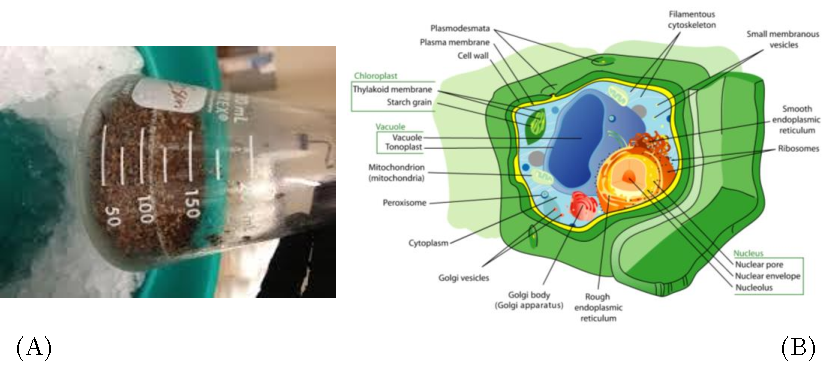
\includegraphics{fig2-1}
    \caption{Examples of capture of information in biology. (A) A flask containing hundreds of individuals of the species drosophila melanogaster. The population is identified with a label on the container. (B) Schema of a  canonical plant cell, similar to the one found in text-books. Parts of interest are annotated with terms, following a descriptive approach. Pictures from Wikipedia.}
    \label{fig2-1}
\end{figure}

\begin{figure}[ht]
    \centering
    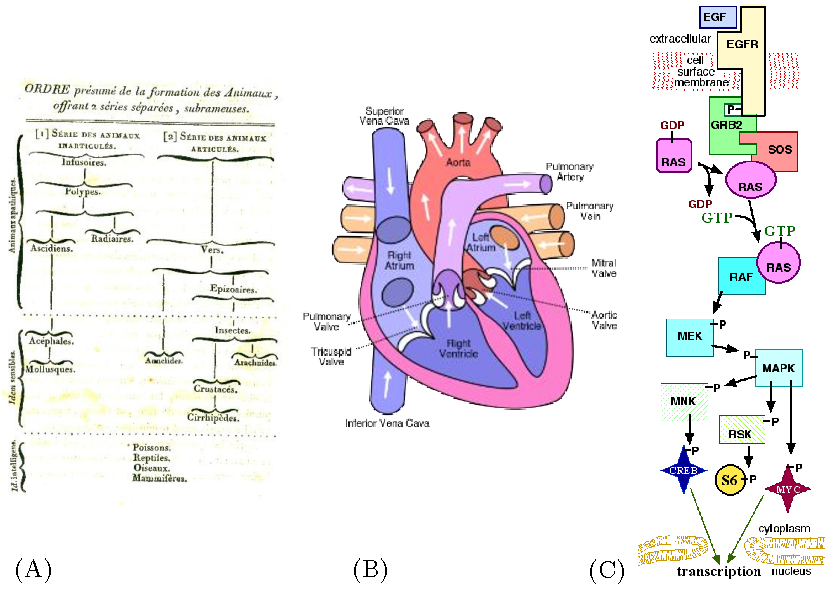
\includegraphics{fig2-2}
    \caption{Formalisation in biomedical sciences. (A) Diagram showing the evolutionary taxonomy of invertebrates. Drawn by Jean-Baptiste Lamarck’s in 1815. (B) Mechanistic illustration of the cardiovascular system. Arrows illustrate the flow of blood and the logical connection between the annotated parts. (C) MAPK/ERK signaling pathway. Schema of the cascade of molecular events leading to activation of transcription factors. The logic of the system is informally captured using arrows, colours and shapes. Images from Wikipedia.}
    \label{fig2-2}
\end{figure}

Nowadays, with the advent of computers and the Internet, known biological entities and concepts are further stored inside public databases. Often, a manual curation step over the published literature improves the consistency and correctness of the data \citep{brooksbank2014european}. The structured information makes it easier for the community to retrieve the data and to perform statistical analyses on it. Nonetheless, this framework is not fully formalised; for example it is not possible to mathematically prove why a drug could be useful for a disease, such as one can logically derive with a series of steps the value of the variable $ x $ out of the following equation: $ 2x = 4 + x $.

How can one further formalise biomedical knowledge to assist the development of new medicines and the study of the living world? A naive approach would try to simplify the system life scientists are working with into a meaningful analogy \citep{lazebnik2002can}. In this regard, I will present how the study of a living organism can be compared to the study of a black box machine, namely a device for which nothing about the internal workings is known (see Figure \ref{fig2-3}).

\begin{figure}[ht]
    \centering
    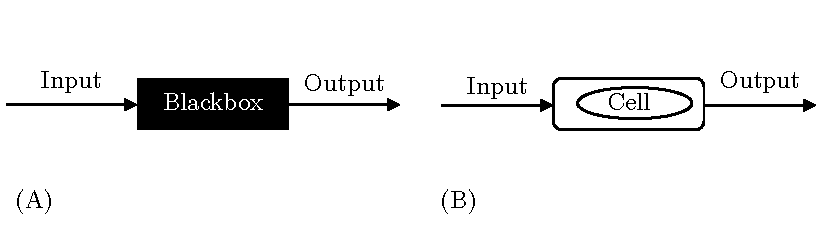
\includegraphics{fig2-3}
    \caption{Blackbox model. (A) Schematic representation of a blackbox. Given an input, an observable output is produced. The internal workings are supposedly not understood. (B) Cells or organism are blackboxes: They can carry various and observable functions from an input, yet the internal workings are not necessarily fully understood.}
    \label{fig2-3}
\end{figure}

\subsubsection{Organisms as complex machines}

From the perspective of drug discovery, an organism (related to organisation) can be broadly simplified as an assembly of molecules functioning as a stable whole. This characteristic makes organisms similar to a machine in the generic sense, which can be described as an assembly of parts functioning to meet a particular goal; in the case of the organism, the intrinsic goal is survival or reproduction. Based on these definitions, biomedical sciences can be seen as the sciences of preventing and repairing dysfunctioning organisms - or molecular machineries.

According to this analogy, the study of a living organism can therefore be compared to the study of a complex black box machine, composed of a large number of physical parts carrying a certain number of internal functions and acting together in an organised fashion.

Now assuming that a certain community has access to such a machine and wants to study it for various reasons, how can it theoretically be done? The analogy becomes insightful at this stage, as there are plenty of complex man-made devices the reader can relate to, and which will serve to illustrate the thought process. I will consider an airplane as example, because it is a complicated device with a straightforward goal: safely flying in the air. A similar exercise can be done with a radio \citep{lazebnik2002can}.

Supposing that a fully functional airplane was found somewhere and the only thing known about it was that the device is capable of flying. The aim is to understand as accurately as possible how the machine works, in order to have enough knowledge to be able to fix it in case it gets broken or malfunctions in the future. In order to address this problem, I argue in favour of a straightforward descriptive approach, in line with the way biological sciences are performed, namely describing the device in as much detail as possible.

The first task done would be to schematise the device, as shown in Figure \ref{fig2-4}-A. Then the fundamental physical parts would get annotated with arbitrary names (\ref{fig2-4}-B). With an increased understanding of the physical modules composing the airplane, it would then be possible to discover the roles played by the various parts of the machinery. Objects would receive functional annotations, namely an explanation of what they do in the overall flying process, as shown on Figure \ref{fig2-4}-C. Up to this step, the system would be characterised as a collection of discrete physical and functional modules, each isolated from one another. Finally, in order to appreciate the machine as a whole, it would become mandatory to link the modules based on their relation types. Figure \ref{fig2-4}-D shows the high level logical organisation of the machine, which integrates the parts to understand the overall process.

\begin{figure}[ht]
    \centering
    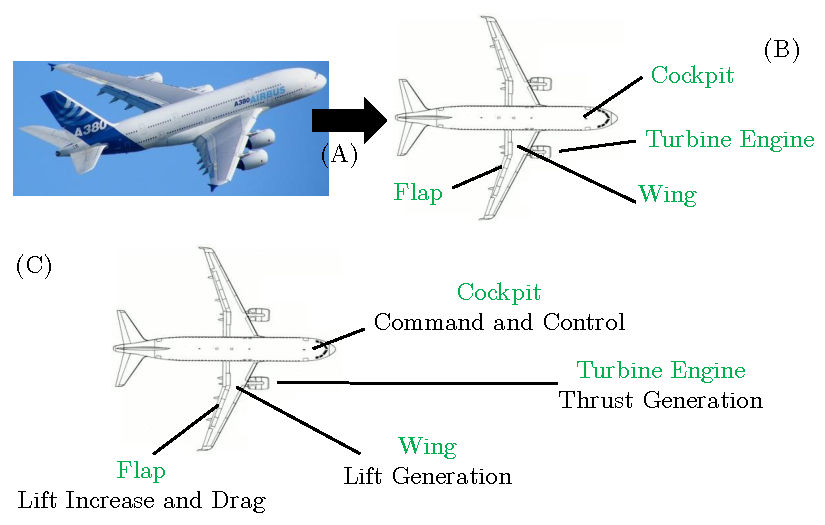
\includegraphics{fig2-4}
    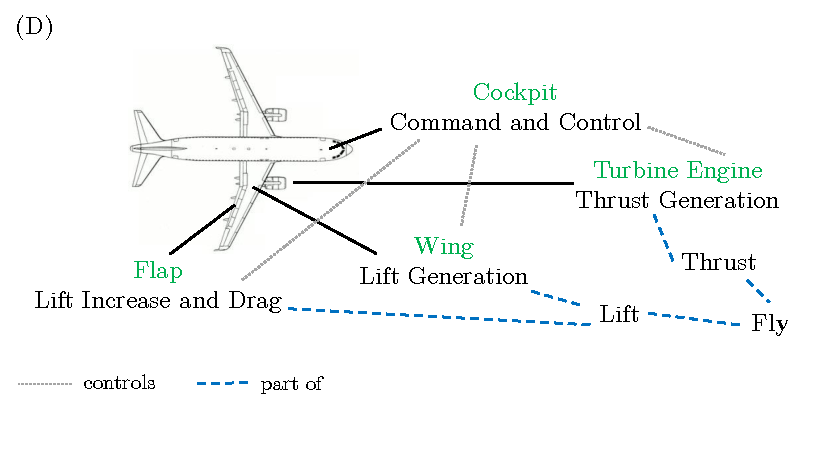
\includegraphics{fig2-4bis}
    \caption{Caption.}
    \label{fig2-4}
\end{figure}

\subsubsection{Organisms as complex machines}

Unveiling the internal logic of the black box machine using this descriptive methodology would later allow extensive querying of the model of the system and simulation of its behaviour. For instance, assuming a problem was identified with the lift of an airplane, preventing it from flying. From the model, it would be possible to retrieve all the known parts directly or indirectly involved in the lift process, derive a list of potentially faulty components and suggest ideas on how to logically repair it and restore its ability to fulfil its primary goal, flying.

The black box machine analogy allows one to better understand the requirements of a formal descriptive framework in order to capture biomedical knowledge. From a drug discovery point of view, organisms can be fundamentally reduced to machines. The descriptive process of studying such machines I presented is analogous to the approach researchers use to study organisms, understand diseases and find treatments for them.

In order to move from an informal characterisation into a defined framework, it is first necessary to determine what is required for a descriptive approach to successfully capture biology. The next section will identify some of the concrete needs for biomedical knowledge, derived from the theoretical model of the molecular black box machine and its study.

\subsection{Requirements for biomedical knowledge formalisation}

In order to be efficiently reused and shared, biomedical knowledge has to be formalised. One way to investigate the living world consists of considering organisms as complex machines; descriptions and annotations of the parts of the machine then help to represent the knowledge and understand better the functioning of the whole device. However, in order to be meaningful, this descriptive approach needs to fulfil a series of criteria introduced in the following section.

\subsubsection{Mathematical framework}

Extending a mathematical field is a key feature of any formal framework. Mathematics help to accurately formulate problems and provide the generic means to solve them. In the case of biomedical knowledge, the ultimate aim is to reduce the burden of diseases for society. To achieve this goal, a formal framework must first be able to capture biological information. Secondly and more importantly, it should be possible to further exploit the framework to deduce and prove assumptions over it. For instance, the mathematical branch of geometry handles questions related to shapes and space. Even if this framework provides only a simplified view of reality, geometry provides the formal means to attest to the validity of a building’s blueprints or optimise land exploitation. Similarly, in the biomedical domain, one should expect to be able to deduce implicit facts or formulate new hypotheses regarding potential treatments directly out of the mathematical formalisation, which is currently not the case. Connecting descriptive biomedical knowledge with mathematics also insures that the framework can benefit from the latest progress in the field. It helps different communities to work together on the same issues from different angles. Formulating biomedical knowledge in mathematical terms also opens the door for computer sciences to assist later on with the implementation of a digital solution.

\subsubsection{Definitions}

The annotation of the parts of the machine requires the usage of a new and specific vocabulary. Words and concepts can be ambiguous, especially when the system analysed is complex such as a living body. A recent illustration of the importance of definitions in biology is the debate over the ENCODE project conclusions \citep{Form_and_function_2013}; different scientists have different interpretations of the word function, which shift the explanation of the results. Semantics, the investigation of the meaning of symbols and words, can assist in this task and help to specify the intended meaning of a concept. Moreover, a formal framework for biomedical knowledge should be able to define any type of things: real-life objects, such as molecule, protein or cell for example. Abstract biological processes like blood coagulation or diseases such as cancer should also be part of the framework, as they are essential concepts in biomedicine. Finally, in order to appreciate the logic of the machine as a whole, it is mandatory to be able to link concepts and words, in order to show how parts of the machinery interact together. The meaning of such relations should be explicit and unambiguous, just as the definitions of concepts.

\subsubsection{Hierarchies and abstraction}

In practice, organisms are probably more analogous to Rube-Goldberg machines than airplanes (see Figure \ref{fig2-5}), with an internal logic sometimes difficult to understand on its own; this results in practice in a tangled network of chemical wiring, which can be abstracted and simplified into functional modules (\cite{hartwell1999molecular}, \cite{ravasz2002hierarchical}, \cite{machado2011modeling}, \cite{fisher2007executable}). Biomedical knowledge has to deal with entities ranging from chemical drugs to high level concepts such as species or biological processes. All these layers have to be integrated and linked in order to understand the machine as a whole. In this regard, it is critical for the formal framework to support abstraction and enable the representation of hierarchical information.

Taxonomies have always been at the heart of biological sciences; take for instance the work of Carl Linnaeus and the Systema Naturae \citep{von1770systema}. Classifications are further used to organize species, protein and chemical families, to name a few examples. Historically speaking, categorical information has provided a good and intuitive framework to capture biomedical knowledge; therefore, any attempt for further formalisation must be able to handle this type of data, as well as to leverage its use.

\begin{figure}[ht]
    \centering
    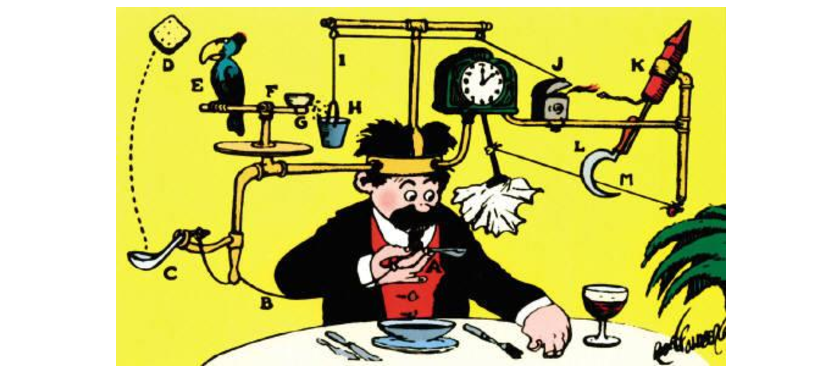
\includegraphics{fig2-5}
    \caption{Rube Goldberg machine: Over-engineered or overdone machine that performs a very simple task in a very complex fashion, usually including a chain reaction \citep{rubewiki}. The picture shows the "Self-Operating Napkin“. When the spoon soup is raised, a cascade of events are triggered ending as the napkin coming toward the man’s face. The task performed is relatively trivial, yet many steps are needed to execute it. Organisms are assumed to be analog to Rube Goldberg machines because of evolution; the internal wiring is not necessarily straightforward and progressively evolved and changed \citep{ravasz2002hierarchical}. Illustration from Wikipedia.}
    \label{fig2-5}
\end{figure}

\subsubsection{Distributed and scalable}

Studying a system as elaborate as an organism requires the collaboration of a large number of persons, working in parallel on different facets of the problem. All these individuals must be able to access and share their knowledge, in order to communicate and be aware of the latest progress. Disseminating information has been usually performed via printed literature, which is being replaced at the time of writing by the World Wide Web and the Internet. This shift of infrastructure allows the processing of more and more information in a digital context, where computers can perform an increasing amount of the work in an automated fashion. This characteristic is particularly interesting for biomedical information, as it is possible to use computers as part of the formalisation process. However, this approach leads to challenges, in particular scaling issues. As organisms are of high complexity, it is therefore important to opt for a formal solution able to cope with problems of large input size. It is assumed that biomedical knowledge will only grow bigger with time, so a mathematical framework should take care of this concern, in order to be future-proof. Finally, it is supposed that biomedical knowledge is and always will be incomplete; in order to be powerful enough, the mathematical formalisation has to able to handle missing information.

\subsubsection{Molecular dynamism}

One of the characteristics of living forms is their dynamism; as organisms are made of molecules, they are subject to the laws of chemistry and molecular dynamics. Organisms can be defined in chemical terms as semi open systems \citep{meng2004modeling}, which emphasises a strong relationship with the environment. Formalisms coming from chemistry, such as conservation of mass \citep{masswiki} or thermodynamics \citep{thermowiki} can represent and solve such systems, yet they are not suited to handle more abstract concepts from the biomedical domain. An ideal formal framework for biomedical knowledge would appreciate the impact and interaction with the environment, yet this requirement is extremely challenging in regards to the number of chemical reactions to be considered \citep{meng2004modeling}. Moreover, the chemical formalisation strongly relies on kinetic parameters to capture behaviour, which makes them vulnerable to missing knowledge. Finally, another concern is the effect of chemical concentration in regards to the function. For instance, the action of a drug strongly depends on its administered dosage. Understanding in detail the biological machinery and deriving correct predictions out of it implies considering molecular dynamics.

Formalising biomedical sciences can be done using a descriptive methodology; this approach has been used since the origin of the field and is an intuitive way to represent biological systems and facts. I presented in this section the theoretical requirements deriving from the descriptive methodology and more generally biomedical sciences. The coming section illustrates how DLs can address some of these requirements in order to mathematically formulate and further use biomedical knowledge.

//TODO under this line must be done

\section{Description logics for biomedical knowledge representation}

DLs are part of a family of formal languages used to represent the knowledge of a domain of interest. The plural form of the word logic indicates that a multitude of languages exist, each one of them characterised by a certain type of expressivity, as it will be seen later in this chapter. The framework evolved from semantic networks (//cite http://dl.acm.org/citation.cfm?id=981256) and inherited its current name around 1980 with the advent of computer systems. DLs are well characterised from a theoretical point of view and implemented in the Web Ontology Language (OWL), a standard supported by the World Wide Web Consortium (W3C). For these reasons and because they address most of the requirements presented before, DLs are an ideal mathematical framework that can be used to formalise some biomedical knowledge.


\subsection{Problem addressed}

aecenas sit amet ligula non dolor varius auctor non quis ligula. Fusce dapibus auctor varius. Praesent tortor ligula, auctor ut dictum eu, rhoncus vitae nunc.

\subsection{Expressivity and complexity}

 libero purus, adipiscing in semper sed, pharetra iaculis.
